\title{Neural Networks - Final Report: Learning Vector Quantization}
\author{Ryan Spangler}
\date{\today}

\documentclass[12pt]{article}

\usepackage{commath}
\usepackage{graphicx}
\usepackage{listings}
\usepackage{amsfonts}

% python highlighting ----------
\usepackage{color}
\usepackage{listings}
\usepackage{textcomp}
\usepackage{setspace}
%\usepackage{palatino}

\renewcommand{\lstlistlistingname}{Code Listings}
\renewcommand{\lstlistingname}{Code Listing}
\definecolor{gray}{gray}{0.6}
\definecolor{green}{rgb}{0.1,0.6,0.3}
\definecolor{orange}{rgb}{0.9,0.7,0.1}
\definecolor{blue}{rgb}{0,0.6,0.8}

\lstnewenvironment{python}[1][]{
\lstset{
language=python,
basicstyle=\ttfamily\footnotesize\setstretch{1},
stringstyle=\color{red},
showstringspaces=false,
alsoletter={1234567890},
otherkeywords={\ , \}, \{},
keywordstyle=\color{blue},
emph={access,and,break,class,continue,def,del,elif,else,%
except,exec,finally,for,from,global,if,import,in,is,%
lambda,not,or,pass,print,raise,return,try,while},
emphstyle=\color{gray}\bfseries,
emph={[2]True, False, None, self},
emphstyle=[2]\color{orange},
emph={[3]from, import, as},
emphstyle=[3]\color{blue},
upquote=true,
morecomment=[s]{"""}{"""},
commentstyle=\color{gray}\slshape,
emph={[4]1, 2, 3, 4, 5, 6, 7, 8, 9, 0},
emphstyle=[4]\color{blue},
literate=*{:}{{\textcolor{blue}:}}{1}%
	{=}{{\textcolor{blue}=}}{1}%
	{-}{{\textcolor{blue}-}}{1}%
	{+}{{\textcolor{blue}+}}{1}%
	{*}{{\textcolor{blue}*}}{1}%
	{!}{{\textcolor{blue}!}}{1}%
	{(}{{\textcolor{blue}(}}{1}%
	{)}{{\textcolor{blue})}}{1}%
	{[}{{\textcolor{blue}[}}{1}%
	{]}{{\textcolor{blue}]}}{1}%
	{<}{{\textcolor{blue}<}}{1}%
	{>}{{\textcolor{blue}>}}{1},%
    frame=fullbox, rulesepcolor=\color{gray},#1
%framexleftmargin=1mm, framextopmargin=1mm, frame=shadowbox, rulesepcolor=\color{blue},#1
}}{}

\setcounter{secnumdepth}{0}

\begin{document}
\maketitle

\section{Abstract}

This paper explores the Linear Vector Quantization (LVQ) neural network paradigm and its application to a real world problem.  Given a set of training data about land use, this experiment proceeds to train the network to optimal performance, then progressively remove features until only the essential features remain.  Using this subset of features, the network is able to be trained to high optimality ($>$ 90\% classification accuracy).  

\section{Introdution/Background on LVQ}

The LVQ is a supervised training algorithm that relies on competition between its PEs to attain a classification of inputs into a predefined set of classes.  During training the incoming vectors are compared against the vectors represented by each PE.  The closest one is considered the ``winner'' and its output is transmitted to the next layer to determine which class the input vector belongs to.  If it is the correct class, the PE is moved closer to the input vector, and if not it is moved away (this is known as ``repulsion'').  After the network has been trained, it performs classification according to the same principles, only the vectors for each PE are no longer moved.  Each pass through the network at this point represents a classification of the vector to one of a certain number of classes, determined by the number of output elements chosen before training.  

The overall effect of the LVQ is ``as if'' the network is optimized to classify its set of presented data according to the classes associated with them, regardless of the nature of the data and without having to have any specific knowledge about the data outside of what classes each training vector belongs to.  

\section{Problem Statement}

The problem for this project is, given the training data set of 52 features and using the LVQ neural network paradigm, discover the smallest subset of features that enables the network to correctly classify the data above 90\% of the time.  It is claimed that 9 features is sufficient for the network to achieve these results, and that even smaller subsets are possible.  My task is to find this minimal subset.

\section{Experimental Process}

The first step was to train an LVQ network with the full set of 52 features.  This was done by creating an LVQ network in NeuralWorks (NW) from the InstaNet menu.  The parameters were as follows:

\begin{center}
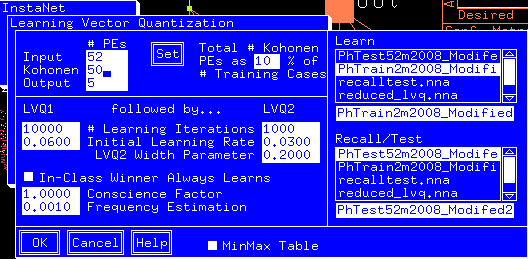
\includegraphics[scale=0.7]{parameters52features.png}
\end{center}

The main notable parameter in this table is the number of Kohonen PE's, which I chose to be 50.  In the documentation of the LVQ it says there must be the same number of competitive layer PE's for each output, so I chose for this experiment to have 10 PE for each of the five outputs.  I was suspicious of this however, so I tried again with 15 to see if this made any difference in the results.  

The parameters for this experiment are given below:

\begin{center}
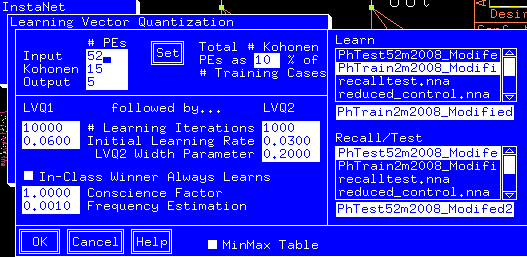
\includegraphics[scale=0.7]{parameters52features15PE.png}
\end{center}

These two runs are compared in order to see what effect having a lower number of PE's has on the effectiveness of the training.  It could be that having too many PE's dilutes the effectiveness of any one PE in making a distinction among data, but on the other hand more PE's could enable the network to perform a wider range of more discriminatory classifications.  

The weight matrix can be viewed in two ways.  In the first, and how the network is trained, the value for each feature is applied to each PE.  These features form an instar, and the PE receives one input from each feature, multiplied by the corresponding weight for that feature to that PE.  So in training, the weight matrix is sliced along the rows to make vectors of distinct feature weights, each of which is then multiplied by the input vector to get the input to each PE.

The other way to look at the weight matrix is to slice it along its columns into vectors of values adopted by a single feature across all presentations.  These vectors supply a complementary perspective, where each of the features is portrayed independently of their relationship to other features.  

The discovery of the critical five features was due to a fortuitous insight.  Since all of the data from the training set was in the positive range, training of salient features (which involved moving the vector for the PE towards the input vector upon winning the competition) would on average increase the weight vector for that feature, if the feature contributed to correctly classifying the input.  Therefore, when I subtract the weight vectors of an untrained network from those of its weights after training, the features corresponding to weight vectors with a positive overall change (sum of elements) were the ones that were critical for the correct classification of the input data.    

Performing this analysis on the data I revealed five features whose total sum of the change in feature-related weights was positive, the rest were all negative.  Reducing the feature set to only these five, I started from a fresh network with only five inputs and trained it from this limited set.  It was unnecessary to go through any intermediate steps as the five presented themselves directly from the study of the change in weights during training.

\begin{center}
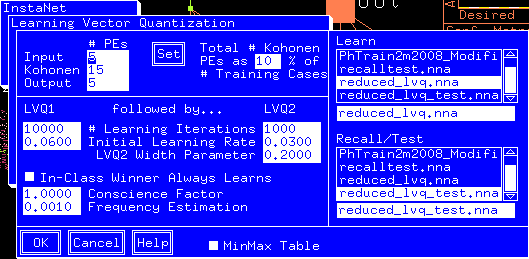
\includegraphics[scale=0.7]{parameters5features.png}
\end{center}

To ensure that this was indeed the correct set of five features I took a control group of five features that all showed negative total weight modification (actually, simply the first five features from the training set) to compare the performance against the five with positive weight modification.  For this run, all parameters were identical except the training and testing data sets:

\begin{center}
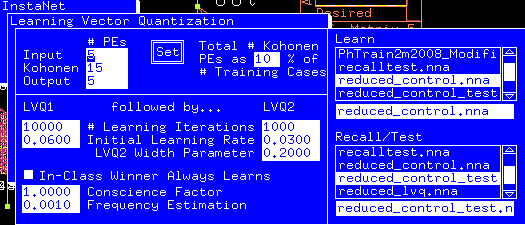
\includegraphics[scale=0.7]{parameters5control.png}
\end{center}

The performance of these two runs was then compared to determine the relative effectiveness of arbitrary features and those that were generally strengthened, and establish the superiority of the chosen five features over an arbitrary selection of five.  

\subsection{Results}

To compare the performance of the networks with different numbers of competitive layer PE's, the run with 50 PE's is compared to the run using only 15 PE's.  Here is NeuralWorks representation of the weight matrix after 11000 learning cycles using 50 PE's with all 52 features:

\begin{center}
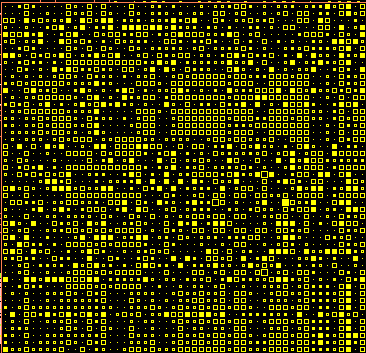
\includegraphics[scale=0.8]{52f50kweights.png}
\end{center}

And here is the same network with only 15 PE's:

\begin{center}
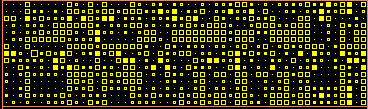
\includegraphics[scale=0.9]{52f15kweights.png}
\end{center}

When the percentage of correctly identified inputs is tracked for each network and overlayed, not much difference is noted:

\begin{center}
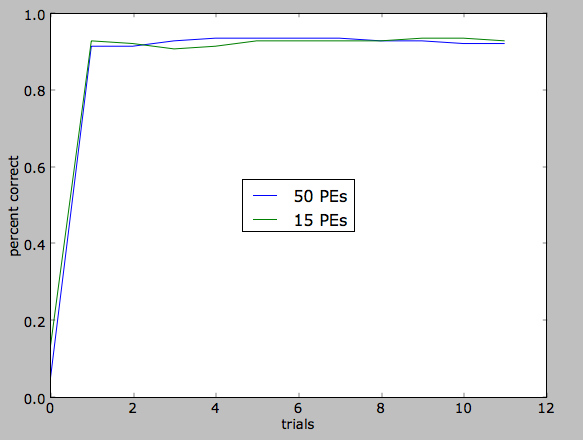
\includegraphics[scale=0.55]{52features.png}
\end{center}

For these graphs, ``trials'' represents the number of snapshots I took of the data.  I sampled the outputs of the network every 2000 training cycles to see how the performance had improved.  It seems arbitrary that the network with 50 PE's ends lower than the one with 15, as it outperforms it for much of the trial.  The network with 15 PE's attained an even 93\% accuracy in test data classification after 11000 presentations of input vectors, whereas the network with 50 PE's reaches only 92.3\%.  In the rest of the experiments I use 15 PE's exclusively.

Numbering the 52 features from 0-51 in the order given in the test data, the critical five features that attained almost 92\% (91.61\%) classification accuracy were:

\begin{itemize}
\item 13
\item 44
\item 45
\item 46
\item 49
\end{itemize}

The other features were more or less irrelevant, or at best redundant.  The presence of all the other features combined contributed only a 1-2\% increase in classification performance.

The five critical features that were discovered were compared with five of the other features to get some kind of sense for how much better the network performed with the critical features than just a random assortment.  The trained weights for the critical features look like this:

\begin{center}
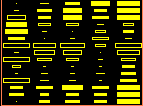
\includegraphics[scale=1.2]{5featuresweights.png}
\end{center}

Whereas for the random assortment of features the weight matrix turned out like this:

\begin{center}
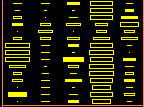
\includegraphics[scale=1.2]{5controlweights.png}
\end{center}

When compared, it is obvious the five features perform better:

\begin{center}
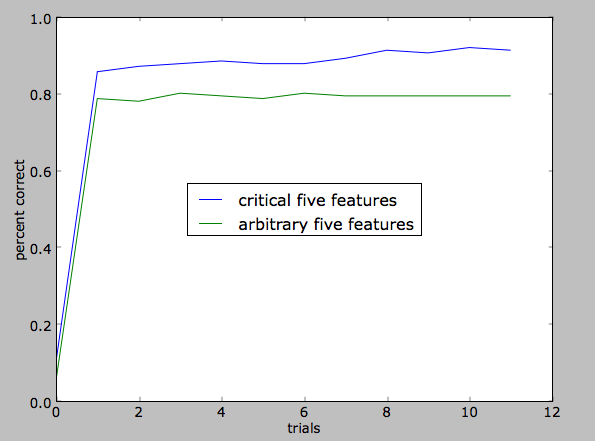
\includegraphics[scale=0.7]{5features.png}
\end{center}

The random assortment of features reaches only a 79\% classification rate, whereas the network trained with the critical five features attains a 91.6\% under the exact same conditions.  This is almost identical to using the entire feature set of 52 values!  It is remarkable that such a high rate can be achieved with such a limited subset of the feature set, though it does take the entire 11000 cycles to raise to that level (which is why I use 11000 cycles for all of the other experiments).  

\section{Conclusion}

Ultimately, finding the ideal subset of five features from the full set of 52 depended on deciphering the message encoded in the values of the weights from each input to the competitive PEs.  The network naturally excluded features that did not contribute to the classification through inhibitory weight modifications.  Only the features that actually correlated to the desired classification scheme were encouraged through weight increases, the others were effectively rendered irrelevant.  

It makes me wonder what the process was for obtaining these features in the first place.  It would be interesting to note what kind of bearing these five critical features had on the categories they were attempting to identify, and why they were so much more effective than any of the other features.  It seems the process of making distinctions among the original data would have a great influence on the applicability of the feature in question.  

I was expecting to have to take many pains to find the relevant nine features required by the assignment, but an early insight allowed me to avoid all of these steps and proceed directly to the critical five, far lower than the nine expected of me!  I feel that the innate architecture of the LVQ was advantageous in this regard, in that it made the weights of the contributing features almost obvious, once the realization was made about how to look at them.  

\section{Data Processing and Plotting Program}

This is the python code I used to process the weights and outputs and plot the performance of the various networks:

\begin{python}[]

from pylab import *

def suffix(n):
    s = str(n)
    p = '0' * (3-len(s))
    return p + s

def pull(filename):
    contents = open(filename).read()
    lines = contents.split("\n")
    lines.pop()
    data = array(map(lambda line: map(lambda x: 
        float(x), line.split(" ")[1:]), lines))

    return data

class NNR:
    def __init__(self, filename):
        self.filename = filename

        contents = open(filename).read()
        lines = contents.split("\n")
        lines.pop()

        self.data = array(map(lambda line: 
            map(lambda x: float(x), line.split("\t")[1:]), lines))

        self.outputs = self.data.shape[1] / 2
        self.expected = self.data[:,:self.outputs]
        self.results = self.data[:,self.outputs:]
        self.diff = self.expected - self.results
        self.mask = self.expected * self.results

        self.strict = map(lambda p: all(map(lambda x: 
            abs(x) < 0.2, p)), self.diff)
        self.loose = map(lambda p: abs(sum(p) - 1.0) < 0.2, self.mask)

        self.error = sum(self.diff)

    def performance(self):
        return float(sum(self.loose)) / float(len(self.loose))

class Series:
    def __init__(self, base, steps, desc):
        self.base = base
        self.steps = steps
        self.desc = desc

        self.nnr = map(lambda x: NNR(base+suffix(x)), range(steps))
        self.data = array(map(lambda d: d.performance(), self.nnr))

    def plot(self):
        plot(self.data, label=self.desc)

class Experiment:
    def __init__(self, series, steps):
        self.series = map(lambda s: 
            Series('phtrain/'+s[0], steps, s[1]), series)
        
    def plot(self):
        xlabel('trials')
        ylabel('percent correct')
        for s in self.series:
            s.plot()
        legend(loc='center')

def run():
    experiment5 = Experiment([('5features', 'critical five'), 
                              ('5control', 'arbitrary five')], 12)
    experiment52 = Experiment([('52features50PE', '50 PEs'), 
                               ('52features15PE', '15 PEs')], 12)
    experiment5.plot()
    return experiment

\end{python}

\end{document}  

